\section{System overview}
The system is designed to have a primary page respesonsible for interactive elements for device selection, room detection, and data collection management. This page interacts with various services including the \texttt{BLEScannerService}, \texttt{RssiDataCollector}, \texttt{RssiDataHandler}, and \texttt{BLEAdvertisementScanner}, to carry out device scanning, data collection, and processing.
These services are connected in an event driven manner, which can be partitioned into several stages, where services are activated based on the input from the user interface. 
Figure \ref{fig:StateDiagram} is a state diagram illustrating the different stages. 

\begin{figure}[H]
    \centering
    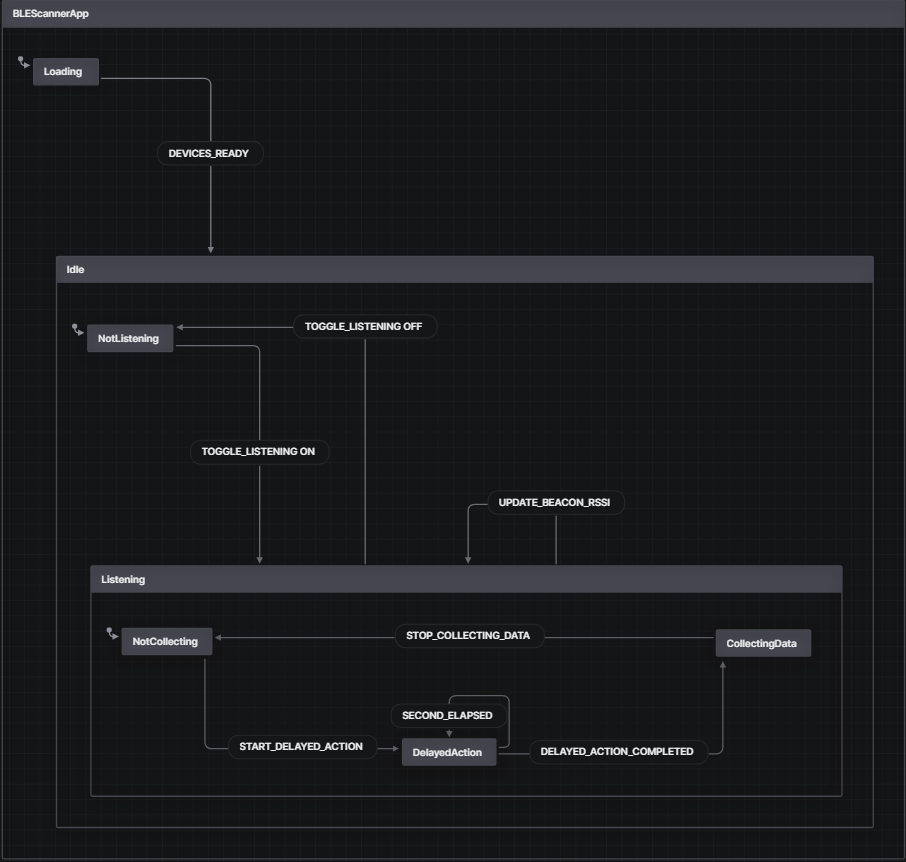
\includegraphics[width=0.8\textwidth]{images/StateDiagram.png}
    \caption{A state diagram illustrating the event propagation}
    \label{fig:StateDiagram}
\end{figure}


\subsection{Blazor Component for BLE Device Monitoring and Analysis}

Upon initialization, the component injects the \texttt{BLEScannerService} and establishes event handlers for device scanning, beacon advertisement updates, and RSSI data updates. The \texttt{RssiDataCollector} and \texttt{RssiDataHandler} instances are responsible for managing the collection and processing of RSSI data, respectively. The \texttt{advertisementScanner} object allows the component to listen for BLE advertisements and update beacon RSSI values accordingly.

The Blazor component presents an interface for users to select available devices for monitoring, initiate or terminate the listening process, and manage the collection of RSSI data. The listening process is triggered by the \texttt{Listen} method of the \texttt{RssiDataCollector} class, which employs a periodic timer to periodically collect data. The component also provides an interface to set the room's label and a threshold for determining whether a device is inside or outside the room.

When the user initiates the data collection process, a countdown timer (represented by the \texttt{DelayedActionExecutor} class) is displayed, and the actual data collection begins after the countdown elapses. The component then displays the current status of whether the monitored devices are inside or outside the room, based on the calculated distances and the specified threshold.

Upon completion of the data collection process, the collected data is written to a JSON file for further analysis. The \texttt{IPromptService} is used to handle user prompts and display relevant information during the execution of the program.
